\capitulo{3}{Conceptos teóricos}

Para la compresion de este proyecto, se deben conocer los siguientes conceptos:

\section{Object Detection}

El Object Detection \cite{objectDetect} es un técnica de vision por ordenador que permite localizar imágenes y/o vídeos. Estos algoritmos se aprovechan del aprendizaje automático o del profundo 
con el objetivo de obtener resultados significativos, es decir, intentan replicar la inteligencia humana a la hora de reconcoer un objeto.
Esta técncia esta cogiendo mucha importancia en los últimos años, obteniendo un papel muy importante en casos de uso de seguridad, transporte, médicos...\\
Usandose en casos cómo:
\begin{list}{\textbullet}{ %
    \addtolength{\itemsep}{-2mm} %
    \setlength{\itemindent}{2mm}}
    \item \textbf{Conducción autónoma:} Este tipo de vehiculos necesitan detectar los objetos para poder reconocer las señales, así como a los peatones, vehículos...
    \item \textbf{Detección de carasterísticas médicas:} Los diagnósticos médicos dependen en gran medida del estudio de imágenes, escaneos y fotografías. Por eso mismo, la detección de objetos en tomografías computarizadas y resonancias magnéticas se ha vuelto especialmente útil a la hora de detectar enfermedades. 
\end{list}

\begin{figure}[!h]
		\centering
		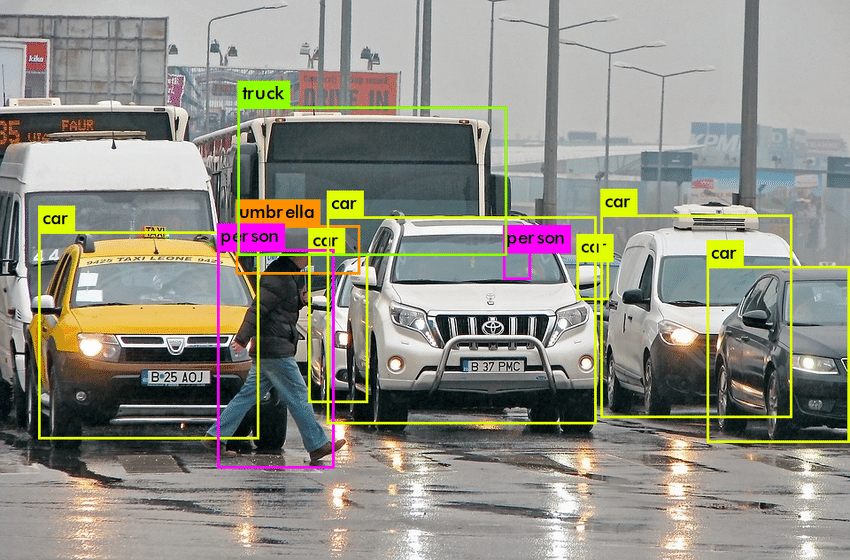
\includegraphics[width=0.6\textwidth]{object_detection}
		\caption{Detección de objetos \cite{imgOD}}\label{fig:object_detection}
\end{figure}

\section{Deep Learning} 

El Deep Learning \cite{deepLearning} es una rama del Machine Learning, donde los algoritmos inspirados en el funcionamiento del cerebro humano (redes neurnales) aprenden a partir de 
grandes cantidades de datos y tratan con un alto número de unidades computacionales.

Gracias a la neurociencia, el estudiio de casos clínicos de daño cerebral sobrevenidoy los avances en diagnóstico por imágenes sabemos que hay centros específicos del lenguaje, que 
existen redes especializadas en detectar diferentes aspectos de la visión, como los bordes, la simetría, áreas relacionadas con el reconocimiento de rostros y las expresiones emociales de los mismos.
Los módelos de Deep Learning imitan estas características de arquitectura del sistema nervioso, permitiendo que dentro del sistema global haya redes de unidades de proceso que se especialicen en la detección
de determinadas características que se encuentran ocultas en los datos. Dicho enfoque, ha permitido obtener mejores resultados si los comparamos con la redes monolíticas de neuronas artificiales

\begin{figure}[!h]
    \centering
    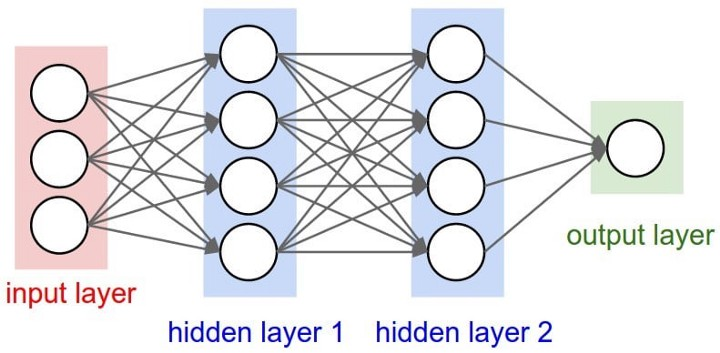
\includegraphics[width=0.5\textwidth]{deep_learning_network}
    \caption{Red neuronal convolucional \cite{imgDL}}\label{fig:deep_learning_network}
\end{figure}

\clearpage

\section{Algoritmo de detección}
A parte de tener claro el lenguaje que se quiere utilizar, otra característica a tener en cuenta es elegir el \textit{algoritmo de detección} en el que se va a basar el modelo.
Existen diferentes algoritmos:
\begin{list}{\textbullet}{ %
    \addtolength{\itemsep}{-2mm} %
    \setlength{\itemindent}{2mm}}

    \item \textbf{CNN:} \textit{(Convolutional Neuronal Network)} es la opción maás básica que se puede escoger,ya que se parte de una red neuronal convolucional \cite{cnn} la cuál itera la imagen hasta devolver las posiciones de los objetos que detecta.
    
    Está opción trae consigo diferentes inconvenientes:
    \begin{list}{\textbullet}{ %
        \addtolength{\itemsep}{-2mm} %
        \setlength{\itemindent}{2mm}}
        \item Si la imagen detecta varios objetos, situados en zonas opuestas, ¿cuántos píxeles tendremos que desplazarnos en cada dirección?.
        \item El tiempo de cómputo es variable, pudiendo llegar a ser muy largo, ya que por cada movimiento implica una clasificación individual con la red.
        \item Deetectar un objeto dentro de la red, no indica que se poseen los valores 'x' e 'y' de su posición.
        \item Si por un casual el desplazamiento de píxeles que se realiza es muy pequeño, podríamos estar detectadndo el mismo objeto múltiples veces.
        \item Si dos objetos se encuentran muy juntos, se podrían llegara a detectar como un único objeto.    
    \end{list}
    
    \item \textbf{R-CNN:} \textit{(Region Based Convolutional Neural Networks)} surgen en el año 2014, con la siguiente propuesta: determianr primero las regiones de interés de la imagen y después realizar la clasificación de imágenes sobre dichas áreas usando una red preentrenada.\cite{r-cnn}
    Esto implica, que haya un primer algoritmo que detecte las áreas de interés de la imagen, las cuáles pueden ser muchas y de diversos tamaños. Seguidamente, se pasán las diferentes regiones por la CNN, validandose las clases correctas mediante un clasificador bianrio, de tal forma, que se eliminarán
    las que tenga un bajo nivel de confianza. Por último, se ajustaría la posición mediante un regresor.
    
    \imagen{r-cnn-regions}{Pasos de la detección en R-CNN \cite{faster_rcnn}}

    \item \textbf{Fast R-CNN / Faster R-CNN:} Son dos algoritmos que surgen como mejora a R-CNN \cite{faster_rcnn}:
    \begin{list}{\textbullet}{ %
        \addtolength{\itemsep}{-2mm} %
        \setlength{\itemindent}{2mm}}
        \item \textbf{Fast R-CNN:} mejora el algoritmo inicial reutilizando algunso recursos, como las \textit{features} extraídaa por la CNN, de tal forma que se agiliza el entreno y la detección de las imágenes.
        Esta red, posee también mejoras en el cálculo del IoU \textit{(Intersection Over Union)} y en la función de \textit{Loss}. Pero a pesar de esto, no tiene mejoras drásticas en la velocidad de entrenamiento y en la detección.
        \imagen{fast-RCNN}{Arquitectura red Fast-RCNN \cite{faster_rcnn}}
        \clearpage
       \item \textbf{Faster R-CNN:} logra una mejora de velocidad al integrar el algoritmo de \textit{region proposal} \cite{region_proposal} sobre la propia CNN.
       Además aperece el concepto de usar \textit{anchors} fijos, lo cuál consiste en usar tamaños pre calculados para la detección de obejtos de la red.
       \imagen{fasterRCNN}{Arquitectura red Faster-RCNN \cite{imgFasterRCNN}}
    \end{list}

    \item \textbf{YOLO:} surge en 2016, su nombre viene formado por las siglas de \textit{You Only Look Once} \cite{yolov4}.
    Esta red, como su propio nombre indica hace una única pasada a la red y detecta todos los obejtos para los que ha sido entrenada para clasificar, al realizar un único vistazo obtiene velocidades muy buenas en equipos que no son necesariamente potentes. Lo cuál permite, detecciones en tiempo real de cientos obejtos de forma simúltanea y su ejecución en dispositivos móviles.  
\end{list}
Debido a esto, el modelo escogido ha sido YOLO y en su versión 4, la cuál fue lanzada en Abril del año 2020.

\imagen{resultsYOLOv4}{Comparativa resultados Dataset COCO \cite{imgResultsYOLO}}

\section{YOLO}

You Only Look Once (YOLO) \cite{yolov4} es un algoritmo de detección que usa Deep Learning y CNN para ello, como su nombre indica sólo necesita mirar la imagen una única vez, de tal forma que la detección es mucho más rápida que en otros algoritmos, pero a cambio de sacrificar rendiemiento a la hora de predecir.
Para llevar a cabo la detección, divide la imagen en una cuadríucla de SxS (imagen de la izquierda). Por cada cuadríucla, predice N posibles "bounding boxes" y calcula la probabilidad de cada una de ellas, es decir, en total se predicen SxSxN cajas diferentes (la gran mayoria con una probabilidad muy baja) (imagen del centro). 
Por último, se eliminan las cajas que estan por debajo de un límite, conocido este como non-max-suppression, de tal forma, que se eliminan los objetos detectados por duplciado, dejando los que poseen un mayor valor de predicción (imagen de la derecha).

\imagen{yolo}{Explicación YOLO \cite{yolov4}}

Para entrenar un modelo, basado en el algoritmo YOLO, tendremos que tener las imégenes con las que vamos a entrenar etiquedas con un contenido como el siguiente:

\imagen{formato_yolo}{Representación del contenido etiquetado YOLO}

El primer parámetro representa el id de la clase, es decir, cuando se etiquetan las imágenes se creara un fichero llamado classes.txt, con los nombres de todas las clases que se han etiquetado para el modelo.
El segundo representa la distancia desde la coordenada 'x' al centro, mientras que el tercero hace lo propio desde la coordenada 'y'.
El cuarto parámetro representa el ancho de la anotación, es decir, el ancho del recuadro que conforma la anotación, el último párametro representa el alto de la anotación.

YOLO utiliza una red CNN llamada Darknet, aunque puede ser utilizada cualquier otra red convolucional a la hora de entrenar. Además, YOLO utiliza las redes convolucionales al final de la cadena, sin necesidad de tener que convertir a una red \textit{tradicional.}
La principal cr´tica que tiene es que a pesar de ser rápida, obtiene peores resultados que las redes \textit{R-CNN}, pero con el paso del tiempo las nuevas versiones que se han lanzado se centran en mejorar dicha precisión en los \textit{bounding boxes}, respetando su eficacia.

La arquitectura de la red se basa en una red convolucional \textbf{GoogLeNet} \cite{googlenet}, la cuál consta de 24 capas convolucionales. Enbebe en su salida tanto la parte que clasifica la imágenes como la de posicionamiento y tamaño de los objetos.

\imagen{yolo_archichecture}{Arquitectura de la red convoluvional Darknet \cite{imgArqDarknet}}

Por ejemplo, para el \textbf{CocoDataset}, la cuál debe detectar 80 objetos diferentes, nos dará una salida:

\begin{table}[h!]
    \centering
    \begin{tabular}{| c | c | c | c |}
        \hline
        Tamaño Grilla & Cantidad Anclas & Cantidad Clases & Ccore, X, Y, Alto, Ancho \\ \hline
        13*13 & *3* & (80 + & * 5) \\ \hline
    \end{tabular}
    \caption{Salida COCO Dataset}
    \label{tab:salidaYOLO}
\end{table}

\section{Edge Computing}

El Edge Computing \cite{edgeComputing} es un tipo de informática que ocurre, en la ubicación fisica del usuario, en la ubicación de la fuente de los datos o cerca de estas. Permitiendo 
que los usuarios obtengan servicios mas rápidos y fiables.

La ventaja fundamental de esto, es que permite a las empresas analizar los datos que sean importantes casi en tiempo real, un hecho que en áreas como la fabricación, la sanidad,
las telecomunicaciones o la industria financiera, es una necesidad latente y continua.

Las necesidades industriales hacen que esta tecnología cada vez sea más demandada, debido a que en ciertos entornos la única forma de poder automatizar más los procesos, consiste en tratar
de evitar lo máximo posible la comunicación con la nube, consiguiendo reducir las latencias, consumir menos ancho de banda y por su puesto acceder de manera inmediata a análisis y evaluación
del estado los sensores y dispositivos que la constituyen.

\imagen{edge_computing}{Estructura Edge Computing \cite{imgEC}}

\section{Raspberry Pi}

Una Raspberry Pi, \cite{raspberry} es una placa de microordenador, la cuál fue lanzada al mecado en Febrero del año 2012, a manos de una fundación que lleva su mismo nombre, la cuál tenía el objetivo de llevar la informática al máximo número de usuarios.
Esta placa cuenta con un precio bastante asequible, alrededor de unos 35€, la cuál cuenta con su propia sistema operativo, el cuál se encuentra basado en Linux, pero en los últimos años han salido multitud de sistemas operativos, que permiten convertir 
la Raspberry es un dispositivo para diferentes fines, como pueden ser centros multimedia o emuladores de máquinas recreativas.

Con este dispositivo, podemos tener un ordenador portable (no portátil, ya que si o si será necesario tenerla conectada a una toma de corriente para hacerla funcionar), lo cuál nos permite transportarla en sitios pequeños como una mochila o un bolsillo,
convirtiéndola así en el ordenador más asequible y manejable que se puede encontrar en el mercado.

\imagen{raspberry_pi}{Raspberry Pi \cite{imgRP}}

\clearpage